\section{Related Work}

\begin{figure}[t]
    \centering
    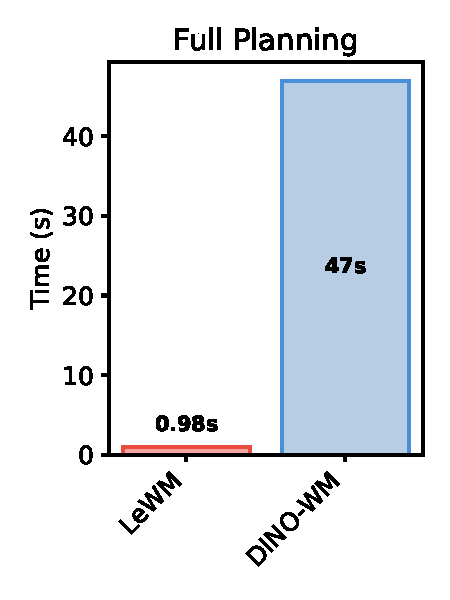
\includegraphics[width=0.32\linewidth]{figs/planning_time.pdf}
    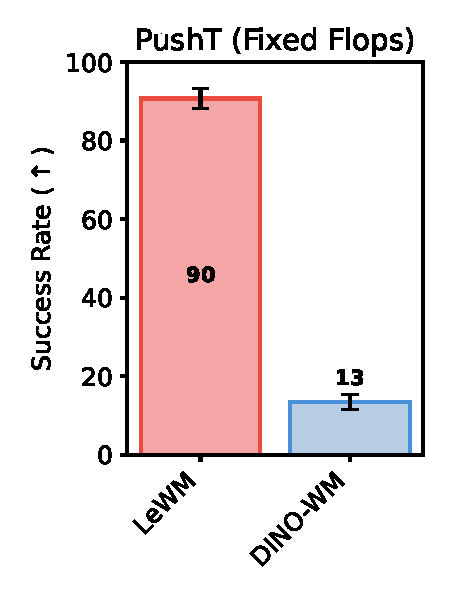
\includegraphics[width=0.32\linewidth]{figs/ctrl-pusht_fixed_flops.pdf}
    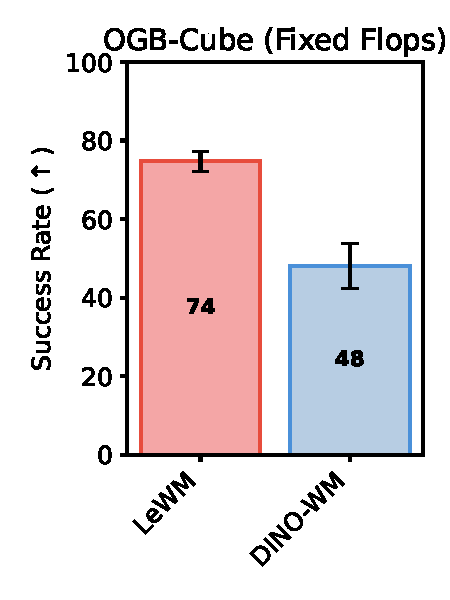
\includegraphics[width=0.32\linewidth]{figs/ctrl-ogb-cube_fixed_flops.pdf}
    \caption{\small \textbf{Planning time and performance under fixed compute.}
    \textbf{Left:} Planning time comparison averaged over 50 runs. Encoding observations with $\sim200\times$ fewer tokens than DINO-WM allows LeWM to achieve planning speeds comparable to PLDM while being up to $\sim50\times$ faster than DINO-WM.
    \textbf{Center–Right:} Planning performance under the same computational budget (fixed FLOPs). LeWM significantly outperforms DINO-WM on Push-T (center) and OGBench-Cube (right). See App.~\ref{appendix:details} for planning setup details.
    }
    \label{fig:planning-time}
\end{figure}

\noindent \textbf{World Models} aim to learn predictive models of environment dynamics from data, enabling agents to reason about future states in imagination. A prominent class of WMs consists of \emph{generative} approaches that explicitly model environment dynamics in pixel space. These action-conditioned generative models act as learned simulators by producing future observations conditioned on past states and actions.
Generative world models have been successfully applied to simulate existing game-like environments. For example, IRIS~\cite{micheli2023transformers}, DIAMOND~\cite{alonso2024diffusion}, $\Delta$-IRIS~\cite{micheli2024efficient}, OASIS~\cite{oasis2024}, and DreamerV4~\cite{hafner2025dreamerv4} model environments such as Minecraft, Counter-Strike, and Crafter, improving policy sample efficiency in reinforcement learning. Other methods generate entirely new interactive simulators, e.g., Genie~\cite{bruce2024geniegenerativeinteractiveenvironments} and HunyuanWorld~\cite{hunyuanworld2025tencent}, while learned simulators have also been applied to robot policy evaluation~\cite{quevedo2025worldgym}.
Importantly, many generative WMs assume access to datasets containing reward signals, enabling joint modeling of dynamics and value-relevant information for downstream reinforcement learning. In contrast, we focus on the reward-free setting, corresponding to the setup considered in the JEPA line of work, which aims at learning generic, task-agnostic world models from observational data without relying on reward supervision.

\noindent \textbf{JEPA} is a framework for learning world models that predict the dynamic evolution of a system in a compact, low-dimensional latent space. Since their introduction by \citet{lecun2022path}, JEPA methods have evolved considerably, differing mainly in their target tasks and in the strategies used to learn non-collapsing representations. One prominent line of work applies JEPA to self-supervised representation learning by predicting the latent embeddings of masked input patches. Examples include I-JEPA~\cite{assran2023self} for images, V-JEPA~\cite{bardes2023v, assran2025v} for videos, and Echo-JEPA and Brain-JEPA~\cite{dong2024brainjepa, munim2026echojepalatentpredictivefoundation} for medical data. These approaches typically employ an exponential moving average (EMA) of the target encoder together with stop-gradient (SG) updates to stabilize training and prevent representation collapse. However, the theoretical understanding of EMA and SG remains limited, as they do not in general correspond to the minimization of a well-defined objective~\cite{ponce2026dual}. A second line of work uses the JEPA recipe for action-conditioned latent world modeling. Some approaches rely on pretrained encoders to obtain representations~\cite{assran2025v, zhou2025dino-wm, goswami2025osviwmoneshotvisualimitation,nam2026causaljepalearningworldmodels}. This avoids collapse but limits the expressivity of representation to the pretrained encoder used. In contrast, PLDM~\cite{sobal2022jointembeddingpredictivearchitectures,sobal2025stresstesting} learns representations end-to-end using VICReg~\cite{bardes2022vicreg} with additional regularization terms, at the cost of known training instabilities and scalability limitations~\citep{balestriero2022contrastive}. Several works further improve stability by incorporating auxiliary signals or architectural components, such as proprioceptive inputs or action decoders~\cite{zhou2025dino-wm, goswami2025osviwmoneshotvisualimitation}. In this work, we propose a stable method for training end-to-end JEPAs directly from raw pixels using a simple two-term loss: a predictive objective on future embeddings and a regularization objective that enforces Gaussian-distributed embeddings~\citep{balestriero2025lejepa}.

\noindent \textbf{Planning with Latent Dynamics.}
World Models~\cite{ha2018recurrent} pioneered learning policies directly from compact latent representations of high-dimensional observations. Some works leverage learned latent dynamics models to train policies using reinforcement learning~\cite{Hafner2020Dream,hafner2020dreamerv2,hafner2023dreamerv3,hafner2025dreamerv4}. In these approaches, the generative world model acts as a simulator in which trajectories are rolled out in imagination, allowing policy optimization to occur largely in imagination in latent space. Once training is complete, the policy is executed directly, and the world model is no longer required at test time.

More recent works instead perform planning directly in the latent space at test time using Model Predictive Control (MPC)~\cite{testud1978model, Hansen2022tdmpc,hansen2024tdmpc,bar2025navigationworldmodels,zhou2025dino-wm,sobal2025stresstesting}. In contrast to imagination-based policy learning, these methods use the world model online to predict the outcomes of candidate action sequences and iteratively optimize them during execution. The model therefore remains part of the control loop at runtime, enabling adaptive decision-making but increasing computational requirements.
